\chapter{Quy hoạch động nâng cao}

\minitoc

\begin{baitap}{Trộn xâu}{https://oj.vnoi.info/problem/stmerge}

Cho 2 chuỗi $X$ gồm $N$ ký tự và $Y$ gồm $M$ ký tự.  

$X = X_1 X_2 \dots X_N$  

$Y = Y_1 Y_2 \dots Y_M$  \\

Hãy trộn 2 chuỗi $X$ và $Y$ này lại thành 1 chuỗi $T$ gồm $N + M$ ký tự sao cho vẫn bảo toàn được thứ tự xuất hiện của các ký tự trong 2 chuỗi.  

Ví dụ:  
$X = X_1 X_2$, $Y = Y_1 Y_2 Y_3$  

Một cách trộn hợp lệ: $T = X_1 Y_1 Y_2 X_2 Y_3$  \\

Xét 2 ký tự kề nhau $T[i], T[i+1]$:  
- Nếu chúng cùng thuộc $X$ hoặc cùng thuộc $Y$ thì chi phí cộng thêm là 0.  
- Nếu một thuộc $X$, một thuộc $Y$ thì chi phí cộng thêm là $cost[p][q]$ với $p, q$ tương ứng vị trí trong $X, Y$.  

\textbf{Input}
\begin{itemize}[noitemsep]
    \item Dòng đầu tiên chứa số $Q$ – số bộ dữ liệu.
    \item Mỗi test:  
    \begin{itemize}
        \item Dòng đầu tiên chứa hai số $N, M$ $(1 \leq N, M \leq 10^3)$.
        \item Dòng tiếp theo chứa $M$ số nguyên – $cost[1][j]$ với $j = 1..M$.
        \item $N-1$ dòng tiếp theo, mỗi dòng chứa $M$ số nguyên – các giá trị $cost[i][j]$ $(1 \leq i \leq N, 1 \leq j \leq M)$.
    \end{itemize}
\end{itemize}

\textbf{Output}  
Với mỗi test, in ra chi phí nhỏ nhất để trộn.

\textbf{Ví dụ}

\begin{sampleio}
1 & 6 \\
2 3 & \\
3 2 30 & \\
15 5 4 & \\
\end{sampleio}

\end{baitap}


\textbf{Phân tích bài toán}

Gọi $f[i][j][k]$ là tổng chi phí nhỏ nhất khi trộn $X[1..i]$ và $Y[1..j]$
\begin{itemize}
    \item $k = 0$: ký tự cuối cùng thuộc chuỗi $X$
    \item $k = 1$: ký tự cuối cùng thuộc chuỗi $Y$
\end{itemize} 

\textbf{Trường hợp cơ sở:}
\begin{itemize}
    \item $f[1][0][0] = 0$
    \item $f[0][1][1] = 0$
    \item $f[i][0][0] = 0$, $\forall i \geq 2$
    \item $f[0][j][1] = 0$, $\forall j \geq 2$
\end{itemize}

Xét $X[1..i]$ và $Y[1..j]$, nếu ký tự cuối cùng thuộc $X$, ta có 2 trường hợp xảy ra:

\begin{itemize}
    \item $f[i][j][0] = f[i - 1][j][1] + cost[i][j]$ : Chuyển từ $Y$ sang $X$ 
    \item $f[i][j][0] = f[i - 1][j][0] + 0$ : Chuyển từ $X$ sang $X$.
\end{itemize}
    
Ngược lại nếu ký tự cuối cùng thuộc $Y$, ta có 2 trường hợp xảy ra:
\begin{itemize}
    \item $f[i][j][1] = f[i][j - 1][0] + cost[i][j]$ : Chuyển từ $X$ sang $Y$
    \item $f[i][j][1] = f[i][j - 1][1] + 0$ : Chuyển từ $Y$ sang $Y$
\end{itemize}

Từ những phân tích trên, ta rút ra được công thức truy hồi tổng quát:


\[
f[i][j][k] = \min \Big( 
    \begin{cases}
        f[i - (k == 0)][j - (k == 1)][k], \\
        f[i - (k == 0)][j - (k == 1)][1 - k] + cost[i][j]
    \end{cases}
    \Big)
\]

\textbf{Kết quả bài toán:} $\min(f[M][N][0], f[M][N][1])$

\textbf{[Groot]:} Ủa, tao để ý nè. Mấy bài trước thì toàn $f[i]$ hay $f[i][j]$ thôi, 
tức là 1 chiều, 2 chiều. Mà qua bài này tự nhiên lại mọc thêm cái $k$, 
thành 3 chiều. Sao biết được bao nhiêu chiều mới đủ? 
Lỡ bài khác phải tới 4–5 chiều thì sao?\\

\textbf{[vuivethoima]:} Vậy nên tao mới đặt bài này trong chương ``QHĐ Nâng cao''. Nói chứ chiều của DP không phải ``càng nhiều càng xịn'', mà là đủ để mô tả trạng thái cần nhớ thôi.  
Ví dụ: 
\begin{itemize}
    \item Bài Ếch chỉ cần nhớ vị trí hiện tại $\Rightarrow$ 1 chiều.
    \item Bài LCS phải nhớ 2 con trỏ đang đứng ở đâu trong $s$ và $t$ $\Rightarrow$ 2 chiều.
    \item Bài này ngoài số ký tự đã dùng ở $X$ và $Y$, 
    còn phải nhớ thêm ký tự cuối cùng thuộc chuỗi nào để tính phí đổi chuỗi $\Rightarrow$ thêm 1 chiều nữa.
\end{itemize}

\textbf{[Groot]:} Vậy tức là số chiều DP = số ``thông tin'' mình cần nhớ lại để tính tiếp hả?\\

\textbf{[vuivethoima]:} Ừ thông minh hơn rồi đó. Mày cần nhớ cái gì thì định nghĩa thêm một chiều cho nó, chứ không phải thích nhét thêm bao nhiêu chiều thì nhét.  
Có mấy bài ``hardcore'' thì thật sự cần 4–5 chiều hay nhiều hơn thiệt, nhưng lúc code người ta hay tìm cách nén trạng thái hoặc rút gọn lại cho nhẹ, bấn quá mới phải đẻ ra nhiều chiều. Hoặc mày cảm thấy cái nhiều chiều đó ngầu thì cứ việc, rồi nộp bài ăn quả TLE xong tạch giải OLP thì đừng có khóc với tao.\\

\textbf{[Groot]:} À hiểu rồi. Không phải ngồi đoán mò số chiều cho vui mà phải xem bài toán bắt mình nhớ những thông tin nào để đi tiếp. Rồi từ đó mới quyết định cần mấy chiều. \\

\begin{lstlisting}[title=\centering\textbf{Cài đặt}]
#include <bits/stdc++.h>
#define int long long
const int oo = 1e18 + 7;
using namespace std;

signed main() {
    int q; cin >> q;
    while (q--) {
        int m, n; cin >> m >> n;
        vector<vector<int>> cost(m + 1, vector<int>(n + 1));
        for (int i = 1; i <= m; i++) {
            for (int j = 1; j <= n; j++) {
                cin >> cost[i][j];
            }
        }

        vector<vector<vector<int>>> f(m + 1, vector<vector<int>>(n + 1, vector<int>(2, oo)));

        for (int i = 1; i <= m; i++) {
            f[i][0][0] = 0;
        }
        for (int j = 1; j <= n; j++) {
            f[0][j][1] = 0;
        }

        for (int i = 1; i <= m; i++) {
            for (int j = 1; j <= n; j++) {
                f[i][j][0] = min(f[i - 1][j][0], f[i - 1][j][1] + cost[i][j]);

                f[i][j][1] = min(f[i][j - 1][1], f[i][j - 1][0] + cost[i][j]);
            }
        }
        cout << min(f[m][n][0], f[m][n][1]) << endl;
    }
}
\end{lstlisting}


\begin{baitap}{Trò chơi với băng số}{https://oj.vnoi.info/problem/linegame}

Có một băng số gồm $n$ ô vuông, đánh số từ 1 đến $n$.  
Ô vuông thứ $i$ ghi một số nguyên dương $a_i$.  

Trong một lượt chơi, người tham gia chọn một dãy các ô $(i_1, i_2, \dots, i_k)$ theo thứ tự từ trái sang phải.  
Điểm số thu được là:
\[
a_{i_1} - a_{i_2} + a_{i_3} - a_{i_4} + \dots + (-1)^{k-1} a_{i_k}
\]

Hãy tính số điểm lớn nhất có thể đạt được từ một lượt chơi.

\textbf{Input}
\begin{itemize}[noitemsep]
    \item Dòng đầu tiên chứa số $n$ $(1 \leq n \leq 10^6)$.
    \item Dòng thứ hai chứa $n$ số nguyên $a_i$ $(1 \leq a_i \leq 10^4)$.
\end{itemize}

\textbf{Output}  
In ra số điểm lớn nhất có thể đạt được.

\textbf{Ví dụ}

\begin{sampleio}
7 & 17 \\
4 9 2 4 1 3 7 & \\
\end{sampleio}

\begin{figure}[h]
    \centering
    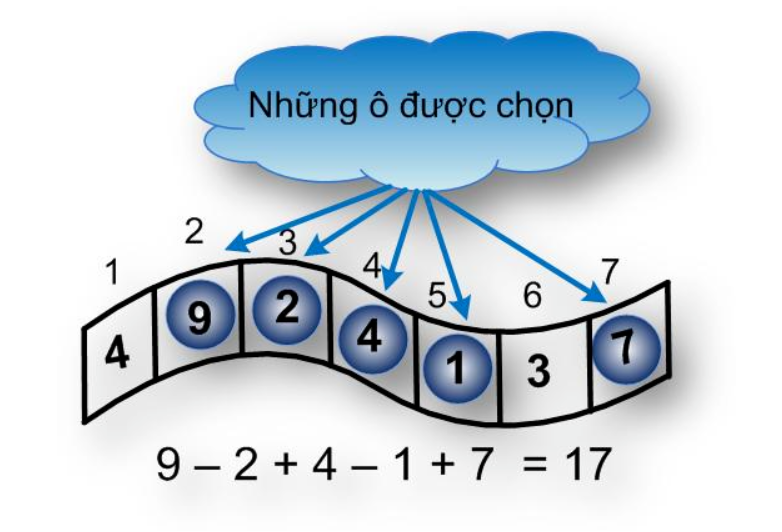
\includegraphics[width=0.4\textwidth]{resource/img/linegame.png}
    \caption{Hình minh họa bài toán.}
\end{figure}

\end{baitap}
\textbf{Phân tích bài toán}  

Gọi $f[i][k]$ là số điểm lớn nhất có thể đạt được khi xét $i$ ô đầu tiên:  
\begin{itemize}
    \item $k = 0$: ô $i$ được chọn và đóng vai trò dấu $+$.
    \item $k = 1$: ô $i$ được chọn và đóng vai trò dấu $-$.
\end{itemize}

\textbf{Trường hợp cơ sở:} $f[1][0] = a[1], \quad f[1][1] = -a[1], \quad f[0][0] = f[0][1] = 0$

Xét ô $i$, ta có các lựa chọn như sau:

\begin{itemize}
    \item Nếu $k = 0$ (ô $i$ mang dấu $+$):
    \begin{itemize}
        \item Nối tiếp từ trạng thái trước đó có dấu $-$: $f[i][0] = f[i-1][1] + a[i]$.
        \item Bắt đầu một dãy mới tại ô $i$: $f[i][0] = a[i]$.
        \item Bỏ qua ô $i$: $f[i][0] = f[i-1][0]$.
    \end{itemize}
    Vậy: $f[i][0] = \max \big( f[i-1][1] + a[i],\ a[i],\ f[i-1][0] \big)$

    \item Nếu $k = 1$ (ô $i$ mang dấu $-$):
    \begin{itemize}
        \item Nối tiếp từ trạng thái trước đó có dấu $+$: $f[i][1] = f[i-1][0] - a[i]$.
        \item Bắt đầu một dãy mới tại ô $i$: $f[i][1] = -a[i]$.
        \item Bỏ qua ô $i$: $f[i][1] = f[i-1][1]$.
    \end{itemize}
    Vậy: $f[i][1] = \max \big( f[i-1][0] - a[i],\ -a[i],\ f[i-1][1] \big)$
\end{itemize}

\textbf{Kết quả bài toán:}  $\max(f[n][0],\ f[n][1])$

\begin{lstlisting}[title=\centering\textbf{Cài đặt}]
#include <bits/stdc++.h>
#define int long long
using namespace std;
const int oo = 1e18 + 7;

signed main() {
    int n; cin >> n;
    vector<int> a(n + 1);
    for (int i = 1; i <= n; i++) {
        cin >> a[i];
    }
    vector<vector<int>> f(n + 1, vector<int>(2, -oo));
    f[1][0] = a[1];
    f[0][0] = 0;

    for (int i = 1; i <= n; i++) {
        f[i][0] = max(f[i][0], a[i]);
        f[i][0] = max(f[i][0], f[i - 1][0]);
        f[i][0] = max(f[i][0], f[i - 1][1] + a[i]);
        
        f[i][1] = max(f[i][1], f[i - 1][1]);
        f[i][1] = max(f[i][1], f[i - 1][0] - a[i]);
    }

    int ans = -oo;

    for (int i = 1; i <= n; i++) {
        ans = max({ans,f[i][0], f[i][1]});
    }
    cout << ans;
}
\end{lstlisting}


\begin{baitap}{Two Paths}{https://lqdoj.edu.vn/problem/twopaths}

Hai anh em An và Bình tham gia một trò chơi thám hiểm trên bảng số \textbf{xTremeMaze}.  

Bảng có kích thước $N \times M$ ($N$ dòng và $M$ cột).  
Mỗi ô $(i,j)$ chứa một số nguyên (có thể âm hoặc dương) biểu diễn điểm kinh nghiệm nhận được khi đi vào ô đó.  

An và Bình bắt đầu tại ô $(1,1)$ và kết thúc tại ô $(N,M)$.  
Mỗi lượt, một người chỉ được đi xuống hoặc sang phải, và không được đi ra ngoài bảng.  
Điểm kinh nghiệm tại ô $(1,1)$ và $(N,M)$ luôn bằng $0$.  

Yêu cầu: tìm tổng điểm kinh nghiệm lớn nhất mà hai anh em đạt được, với điều kiện hai người không đi qua cùng một ô, ngoại trừ ô $(1,1)$ và ô $(N,M)$.

\textbf{Input}
\begin{itemize}[noitemsep]
    \item Dòng đầu tiên chứa hai số nguyên $N, M$ $(2 \leq N, M \leq 200)$.
    \item $N$ dòng tiếp theo, mỗi dòng chứa $M$ số nguyên có giá trị tuyệt đối không quá $100$ — điểm kinh nghiệm của từng ô. 
    \item Bảo đảm $A_{1,1} = A_{N,M} = 0$.
\end{itemize}

\textbf{Output}  
In ra tổng số điểm kinh nghiệm lớn nhất mà An và Bình đạt được.

\textbf{Ví dụ}

\begin{sampleio}
3 3 & 32 \\
0 2 3 & \\
4 5 6 & \\
7 8 0 & \\
\end{sampleio}
\end{baitap}

\textbf{Phân tích bài toán}

Gọi $f[\text{step}][x_1][x_2]$ là tổng số điểm kinh nghiệm lớn nhất khi An và Bình đã thực hiện  
$\text{step} = x + y - 2$ bước, trong đó:
\begin{itemize}
    \item An đang ở vị trí $(x_1, y_1)$ với $y_1 = \text{step} - x_1 + 2$,
    \item Bình đang ở vị trí $(x_2, y_2)$ với $y_2 = \text{step} - x_2 + 2$.
\end{itemize}

Tổng số bước di chuyển là $n + m - 2$, do đó ta duyệt lần lượt các bước $\text{step} = 1 \rightarrow n + m - 2$.

\textbf{Trường hợp cơ sở:} $f[0][1][1] = 0$
\textbf{Công thức truy hồi:}  
Tại mỗi bước, giá trị $f[\text{step}][x_1][x_2]$ được cập nhật từ 4 trạng thái trước đó, ứng với việc An/Bình đi xuống hoặc sang phải:
\[
\begin{aligned}
f[\text{step}][x_1][x_2] = \max \Big\{ 
   & f[\text{step} - 1][x_1 - 1][x_2 - 1], \\
   & f[\text{step} - 1][x_1 - 1][x_2], \\
   & f[\text{step} - 1][x_1][x_2 - 1], \\
   & f[\text{step} - 1][x_1][x_2] 
\Big\} + \text{điểm}
\end{aligned}
\]

Trong đó phần \textit{điểm} được tính như sau:
\[
\text{nếu } (x_1, y_1) = (x_2, y_2) \Rightarrow \text{điểm} = a[x_1][y_1]
\]
\[
\text{ngược lại } \Rightarrow \text{điểm} = a[x_1][y_1] + a[x_2][y_2]
\]

Ngoài ra, cần đảm bảo các điều kiện sau:
\begin{itemize}
    \item $(x_1, y_1)$ và $(x_2, y_2)$ phải nằm trong bảng.
    \item Nếu $(x_1, y_1) = (x_2, y_2)$ thì đó chỉ có thể là ô đích $(n,m)$.
\end{itemize}

\textbf{Kết quả bài toán:} $f[n + m - 2][n][n]$\\

\textbf{[Groot]:} Ê sao phức tạp vậy, tao vừa nghĩ ra cái này. Sao không chơi thẳng $f[x_1][y_1][x_2][y_2]$ luôn?  
Hai thằng đi đâu thì mình lưu hết bốn toạ độ, rõ ràng dễ hiểu, hạnh phúc, thành công, khai phóng vcđ.\\

\textbf{[vuivethoima]:} Ừ, ý tưởng đó là cách tự nhiên nhất, cũng đúng luôn.  
Nhưng nó hoang dã vl, mày thử coi: $N, M$ tối đa 200.  
Nếu làm 4D thì số trạng thái là $200^4 \approx 1.6 \times 10^9$.  
Với mỗi trạng thái lại duyệt 4 cách đi tiếp, thì TLE chếc cụ ấy.\\

\textbf{[Groot]:} À, tức là dễ viết nhưng chậm. Vậy thì cái trick ở đây là gì?\\

\textbf{[vuivethoima]:} Trick là ``đồng bộ bước đi''.  
Mỗi lần cả An lẫn Bình đi thêm 1 bước, thì tổng chỉ số $x+y$ của họ đều tăng lên đúng 1.  
Nói cách khác, sau $\text{step}$ bước thì $x_1+y_1 = x_2+y_2 = \text{step}+2$.  
Vậy là từ 4 toạ độ $(x_1,y_1,x_2,y_2)$ mình rút gọn còn 3 thông tin: $(\text{step}, x_1, x_2)$.  
Khi đó $y_1, y_2$ tính lại được từ $\text{step}$.\\

\textbf{[Groot]:} À ha, nên mới có công thức $y_1 = \text{step} - x_1 + 2$,  
$y_2 = \text{step} - x_2 + 2$ đó hả. Nhờ vậy bộ nhớ giảm từ $O(N^2M^2)$ xuống $O((N+M)N^2)$, đủ chơi với cái giới hạn bài cho.\\

\textbf{[Groot]:} Vậy có khi nào gặp bài mà không nén được như vầy, bắt buộc phải chơi 4D không?\\

\textbf{[vuivethoima]:} Chắc có, nếu hai thực thể di chuyển độc lập mà không có ràng buộc ``đồng bộ'' giữa chúng thì đúng là phải 4D, tao nghĩ vậy? 

\begin{lstlisting}[title=\centering\textbf{Cài đặt}]
#include <bits/stdc++.h>
#define int long long
const int oo = 1e9 + 7;
using namespace std;


signed main() {
    int n, m; cin >> n >> m;
    vector<vector<int>> a(n + 1, vector<int>(m + 1));
    for (int i = 1; i <= n; i++) {
        for (int j = 1; j <= m; j++) {
            cin >> a[i][j];
        }
    }

    vector<vector<vector<int>>> f(n + m, vector<vector<int>>(n + 1, vector<int>(n + 1, -oo)));

    f[0][1][1] = 0;

    for (int step = 1; step <= n + m - 2; step++) {
        for (int x1 = 1; x1 <= n; x1++) {
            int y1 = step - x1 + 2;
            if (y1 <= 0 || y1 > m) continue;
            for (int x2 = 1; x2 <= n; x2++) {
                int y2 = step - x2 + 2;
                if (y2 <= 0 || y2 > m) continue;

                int val = -oo;
                val = max(val, f[step - 1][x1 - 1][x2]);
                val = max(val, f[step - 1][x1][x2 - 1]);
                val = max(val, f[step - 1][x1 - 1][x2 - 1]);
                val = max(val, f[step - 1][x1][x2]); 


                if (x1 == x2 && y1 == y2 && (x1 != n || y1 != m)) continue;

                if (x1 == x2 && y1 == y2)
                    val += a[x1][y1];
                else
                    val += a[x1][y1] + a[x2][y2];
                f[step][x1][x2] = val;
            }
        }
    }
    cout << f[n + m - 2][n][n];
}
\end{lstlisting}

\begin{baitap}{IOI07 Miners}{https://oj.vnoi.info/problem/nkminers}

Có hai mỏ than, mỗi mỏ có một nhóm thợ mỏ làm việc. Khai thác than là công việc vất vả, do đó các thợ mỏ cần thực phẩm để hoạt động. Mỗi khi một đợt vận chuyển thực phẩm đến mỏ, các thợ mỏ sẽ khai thác được một lượng than nào đó. Có 3 loại thực phẩm được vận chuyển: thịt (M), cá (F) và bánh mì (B).

Mỗi đợt vận chuyển thực phẩm được đưa đến một trong hai mỏ, và sản lượng than của đợt đó phụ thuộc vào số loại thực phẩm khác nhau trong hai đợt liên tiếp mà mỏ đó nhận được:
\begin{itemize}
    \item Nếu các đợt vận chuyển cùng một loại thực phẩm $\Rightarrow$ 1 đơn vị than
    \item Nếu có 2 loại thực phẩm khác nhau $\Rightarrow$ 2 đơn vị than
    \item Nếu có 3 loại thực phẩm khác nhau $\Rightarrow$ 3 đơn vị than
\end{itemize}

Các đợt vận chuyển không thể chia nhỏ, và tất cả thực phẩm trong một đợt phải gửi đến một trong hai mỏ. Có thể gửi tất cả các đợt đến một mỏ.

Hãy tìm cách phân chia các đợt vận chuyển sao cho tổng lượng than khai thác được từ hai mỏ là lớn nhất.

\textbf{Input}
\begin{itemize}[noitemsep]
    \item Dòng đầu tiên chứa số nguyên $N$ $(1 \leq N \leq 10^5)$ — số đợt vận chuyển.
    \item Dòng thứ hai chứa xâu $S$ độ dài $N$, mỗi ký tự là một trong \{M, F, B\}.
\end{itemize}

\textbf{Output}  
In ra tổng lượng than lớn nhất có thể khai thác.

\textbf{Ví dụ}

\begin{sampleio}
6 & 12 \\
MBMFFB & \\ \hline
16 & 29 \\
MMBMBBBBMMMMMBMB & \\
\end{sampleio}
\end{baitap}

\textbf{Phân tích bài toán}

Gọi $f[i][a_1][a_2][b_1][b_2]$ là tổng lượng than lớn nhất có thể sản xuất được sau $i$ đợt vận chuyển, trong đó:
\begin{itemize}
    \item $a_1, a_2$ là hai loại thực phẩm gần nhất mỏ 1 đã nhận (Hiện tại là $a_1$, ngày hôm trước là $a_2$).
    \item $b_1, b_2$ là hai loại thực phẩm gần nhất mỏ 2 đã nhận (Hiện tại là $b_1$, ngày hôm trước là $b_2$).
    \item Giá trị của mỗi loại: $0$ (không có), $1$ (M), $2$ (F), $3$ (B).
\end{itemize}

\textbf{Trường hợp cơ sở:}

Giả sử thực phẩm đầu tiên là loại $t = \texttt{code}(s[1])$, ta có:
\begin{align*}
f[1][t][0][0][0] &= 1 \quad \text{(gửi đến mỏ 1)} \\
f[1][0][0][t][0] &= 1 \quad \text{(gửi đến mỏ 2)}
\end{align*}

Với $i \geq 2$, giả sử loại thực phẩm hiện tại là $c = \texttt{code}(s[i])$, ta có hai lựa chọn:

\begin{itemize}
    \item \textbf{Chuyển đến mỏ 1}:
    \[
    f[i][c][a_1][b_1][b_2] = \max(f[i][c][a_1][b_1][b_2], f[i - 1][a_1][a_2][b_1][b_2] + \texttt{energy}(c, a_1, a_2))
    \]

    \item \textbf{Chuyển đến mỏ 2}:
    \[
    f[i][a_1][a_2][c][b_1] = \max(f[i][a_1][a_2][c][b_1], f[i - 1][a_1][a_2][b_1][b_2] + \texttt{energy}(c, b_1, b_2))
    \]
\end{itemize}

Trong đó, hàm \texttt{energy}(a, b, c) là hàm đếm số loại thực phẩm khác nhau trong 3 ngày gần nhất:
\[
\texttt{energy}(a, b, c) = \left| \{a, b, c\} \setminus \{0\} \right|
\]


\textbf{Kết quả bài toán:} 
\[
\max_{a,b,c \in \{0,1,2,3\}} f[n][a][b][c]
\]

\begin{lstlisting}[title=\centering\textbf{Cài đặt}]
#include <bits/stdc++.h>
#define int long long
const int oo = 1e9 + 7;
using namespace std;

int code(char c) {
    return (c == 'M' ? 1 : (c == 'F' ? 2 : (c == 'B' ? 3 : 0)));
}

int energy(int a, int b, int c) {
    return (a != 0) + (b != 0 && b != a) + (c != 0 && c != a && c != b);
}

signed main() {
    ios_base::sync_with_stdio(0); 
    cin.tie(0), cout.tie(0);
    int n; cin >> n;
    vector<char> s(n + 1);
    for (int i = 1; i <= n; i++) cin >> s[i];

    int f[n + 1][4][4][4][4];
    for (int i = 0; i <= n; i++)
        for (int a1 = 0; a1 < 4; a1++)
            for (int a2 = 0; a2 < 4; a2++)
                for (int b1 = 0; b1 < 4; b1++)
                    for (int b2 = 0; b2 < 4; b2++)
                        f[i][a1][a2][b1][b2] = -oo;

    int t = code(s[1]);
    f[1][t][0][0][0] = 1;
    f[1][0][0][t][0] = 1;

    for (int i = 2; i <= n; i++) {
        int cur = code(s[i]);
        for (int t1 = 0; t1 <= 3; t1++) {
            for (int t2 = 0; t2 <= 3; t2++) {
                for (int t3 = 0; t3 <= 3; t3++) {
                    for (int t4 = 0; t4 <= 3; t4++) {
                        f[i][cur][t1][t3][t4] = max(f[i][cur][t1][t3][t4],
                                                    f[i - 1][t1][t2][t3][t4] + energy(cur, t1,t2));
                        
                        f[i][t1][t2][cur][t3] = max(f[i][t1][t2][cur][t3],
                                                    f[i - 1][t1][t2][t3][t4] + energy(cur,t3,t4));
                    }
                }
            }
        }
    }


    int ans = 0;
    for (int a1 = 0; a1 < 4; ++a1)
        for (int a2 = 0; a2 < 4; ++a2)
            for (int b1 = 0; b1 < 4; ++b1)
                for (int b2 = 0; b2 < 4; ++b2)
                    ans = max(ans, f[n][a1][a2][b1][b2]);
    cout << ans;
}
\end{lstlisting}

\textbf{[Groot]:} Ủa, nhưng tao coi lời giải trên mạng thấy có người làm 3 chiều, có người 4 chiều thôi à. Sao mày lại dựng hẳn tới 5 chiều? Có dư thừa gì không?\\

\textbf{[vuivethoima]:} Ờ thì cách tao viết là kiểu full state - giữ luôn 2 món gần nhất của mỗi mỏ. Đảm bảo tính đúng, nhưng hơi minh béo. \\

\textbf{[Groot]:} Vậy sao mày không làm tối ưu hơn, cách mày cài đặt tốn $4^4 \times 10^5$ ô nhớ lận. Viết kiểu đó làm cái gì cho tốn bộ nhớ?\\

\textbf{[Groot]:} Mày coi thử cách giảm chiều của tao bên dưới oke hông?\\

\textbf{Phân tích bài toán (2):}

Gọi $f[i][a][b][c]$ là tổng lượng than lớn nhất có thể sản xuất được sau $i$ đợt vận chuyển, trong đó:
\begin{itemize}
    \item Mỏ vừa nhận đợt $i$ (gọi là mỏ \textit{đang hoạt động}) có hai loại thực phẩm gần nhất là $(s[i], a)$, tức $s[i]$ là loại hiện tại, $a$ là loại liền trước đó.
    \item Mỏ còn lại có hai loại thực phẩm gần nhất là $(b, c)$.
    \item Giá trị của mỗi loại: $0$ (không có), $1$ (M), $2$ (F), $3$ (B).
\end{itemize}

\textbf{Trường hợp cơ sở:}

Với đợt vận chuyển đầu tiên có loại $t = \texttt{code}(s[1])$, ta có: $f[1][0][0][0] = 1$
vì $\texttt{energy}(t,0,0) = 1$.

\textbf{Công thức chuyển:}

Giả sử ở đợt $i$ hiện tại loại thực phẩm là $c = \texttt{code}(s[i])$, khi xét đến đợt tiếp theo $s[i+1]$ có loại $t = \texttt{code}(s[i+1])$, ta có hai lựa chọn:

\begin{itemize}
    \item \textbf{Tiếp tục chuyển đến mỏ đang hoạt động}:  
    Khi đó hai món gần nhất của mỏ này là $(s[i], a)$, nên điểm cộng thêm là $\texttt{energy}(t, s[i], a)$.  
    Trạng thái mới ở bước $i+1$ sẽ là:
    \[
    f[i+1][s[i]][b][c] = \max\Big(f[i+1][s[i]][b][c],\; f[i][a][b][c] + \texttt{energy}(t, s[i], a)\Big)
    \]

    \item \textbf{Chuyển sang mỏ còn lại}:  
    Mỏ còn lại hiện có hai món gần nhất là $(b, c)$, nên điểm cộng thêm là $\texttt{energy}(t, b, c)$.  
    Sau khi giao, mỏ này trở thành mỏ đang hoạt động với $(t, b)$, còn mỏ cũ trở thành mỏ còn lại với $(s[i], a)$.  
    Do đó:
    \[
    f[i+1][b][s[i]][a] = \max\Big(f[i+1][b][s[i]][a],\; f[i][a][b][c] + \texttt{energy}(t, b, c)\Big)
    \]
\end{itemize}

\textbf{Kết quả bài toán:} 
\[
\max_{a,b,c \in \{0,1,2,3\}} f[n][a][b][c]
\]



\begin{lstlisting}[title=\centering\textbf{Cài đặt}]
#include <bits/stdc++.h>
using namespace std;
const int oo = 1e9 + 7;

int code(char c) {
    return (c == 'M' ? 1 : (c == 'F' ? 2 : (c == 'B' ? 3 : 0)));
}

int energy(int a, int b, int c) {
    return (a != 0) + (b != 0 && b != a) + (c != 0 && c != a && c != b);
}

int main() {
    ios_base::sync_with_stdio(0); 
    cin.tie(0), cout.tie(0);
    int n; cin >> n;
    vector<char> s(n + 1);
    for (int i = 1; i <= n; i++) cin >> s[i];

    int f[n + 1][4][4][4];
    for (int i = 0; i <= n; i++) 
        for (int a = 0; a < 4; a++)
            for (int b = 0; b < 4; b++) 
                for (int c = 0; c < 4; c++)
                    f[i][a][b][c] = -1;
                    
    f[0][0][0][0] = 0;
    f[1][0][0][0] = 1;  
    for (int i = 0; i < n; i++) {
        for (int a = 0; a < 4; a++) {
            for (int b = 0; b < 4; b++) {
                for (int c = 0; c < 4; c++) {
                    if (f[i][a][b][c] == -1) continue;

                    f[i + 1][code(s[i])][b][c] = max(f[i + 1][code(s[i])][b][c], f[i][a][b][c] + energy(code(s[i]), code(s[i + 1]), a));

                    f[i + 1][b][code(s[i])][a] = max(f[i + 1][b][code(s[i])][a], f[i][a][b][c] + energy(code(s[i+1]), b, c));

                }
            }
        }
    }

    int ans = 0;
    for (int a = 0; a < 4; a++) {
        for (int b = 0; b < 4; b++) {
            for (int c = 0; c < 4; c++) {
                ans = max(ans, f[n][a][b][c]);
            }
        }
    }
    cout << ans;
}
\end{lstlisting}

\begin{baitap}{Exam Cheating}{https://codeforces.com/problemset/problem/796/E}

Zane và người mà Zane thích vừa mới bắt đầu hẹn hò! Tuy nhiên, cô gái đang gặp khó khăn với kỳ thi cuối kỳ môn Vật lý, và cần bạn giúp đỡ.

Có n câu hỏi, được đánh số từ $1$ đến $n$. Câu hỏi $i$ sẽ đứng trước câu hỏi $i + 1$ $(1 \leq i < n)$. Mỗi câu hỏi không thể chọn bừa, vì nếu trả lời sai sẽ bị phạt rất nặng. May mắn thay, cô gái đang ngồi giữa hai thiên tài, và cô ấy sẽ quay cóp bài họ.

Tuy nhiên, hai thiên tài cũng có giới hạn. Mỗi người có thể biết hoặc không biết câu trả lời của một số câu hỏi. Dù vậy, những câu trả lời trên bài của họ thì luôn chính xác tuyệt đối.

Để không bị giám thị phát hiện, cô gái chỉ được quay cóp tối đa $p$ lần, mỗi lần nhìn được nhiều nhất $k$ câu hỏi liên tiếp từ bài của một trong hai thiên tài. Khi cô ấy nhìn vào bài một thiên tài, nếu câu hỏi đó có trong bài của họ, cô ấy sẽ chép lại, nếu không thì bỏ qua.

Nhiệm vụ của bạn là giúp cô ấy trả lời đúng được nhiều nhất bao nhiêu câu hỏi.

\textbf{Input}
\begin{itemize}[noitemsep]
    \item Dòng đầu tiên: ba số nguyên $n, p, k$ ($1 \leq n, p \leq 1000$, $1 \leq k \leq \min(n, 50)$).  
    \item Dòng thứ hai: số $r$ — số câu hỏi thiên tài 1 biết, tiếp theo $r$ số nguyên phân biệt $a_1,\dots,a_r$ (tăng dần).  
    \item Dòng thứ ba: số $s$ — số câu hỏi thiên tài 2 biết, tiếp theo $s$ số nguyên phân biệt $b_1,\dots,b_s$ (tăng dần).  
\end{itemize}

\textbf{Output}  
In ra số câu hỏi tối đa mà cô gái có thể trả lời đúng.

\textbf{Ví dụ}

\begin{sampleio}
6 2 3 & 4 \\
3 1 3 6 & \\
4 1 2 5 6 & \\ \hline
8 3 3 & 7 \\
4 1 3 5 6 & \\
5 2 4 6 7 8 & \\
\end{sampleio}

\textbf{Ghi chú}  

Ví dụ 1: Có thể chọn các hành động $(1,1,3)$ và $(2,5,6)$ để trả lời đúng 4 câu hỏi.  

Ví dụ 2: Có thể chọn $(1,3,5)$, $(2,2,4)$ và $(2,6,8)$ để trả lời đúng 7 câu hỏi.  \\

\end{baitap}

\textbf{Phân tích bài toán}\\

Gọi hai thiên tài lần lượt là A và B. \\

Gọi $f[i][j][k_A][k_B]$ là tổng số câu tối đa có thể chép được khi xét $i$ câu trắc nghiệm đầu tiên, ta đã có $j$ đợt chép bài. Và:
\begin{itemize}
    \item Đối với người A: ta đã chép được $k_A$ câu liên tục.
    \item Đối với người B: ta đã chép được $k_B$ câu liên tục.
\end{itemize}

\textbf{Trường hợp cơ sở:} $f[0][0][0][0] = 0$

Nếu $k_A = 0$ và $k_B = 0$: hiện tại câu thứ $i$ của bạn A (hoặc B) không được chép.

\textbf{Kết quả bài toán:} \[\max_{j \leq p, 0 \leq kA, kB \leq k} f[n][j][k_A][k_B]\] \\


\begin{lstlisting}[title=\centering\textbf{Cài đặt}]

\end{lstlisting}

\begin{baitap}{SC6}{Summer Contest 2022}

Cho một dãy số nguyên dương a gồm N số. Bạn hãy chia dãy số trên thành k đoạn, mỗi đoạn gồm một dãy gồm các số ở vị trí liên tục sao cho với mỗi số thuộc đúng một đoạn.  
Gọi $s_1, s_2, \ldots, s_k$ lần lượt là tổng các số trên mỗi đoạn.  

Hỏi bạn cần chia như thế nào để được tổng  
\[
|s_2 - s_1| + |s_3 - s_2| + \ldots + |s_k - s_{k-1}|
\]  
lớn nhất.

\textbf{Dữ liệu đầu vào (SC6.INP):}  
\begin{itemize}
  \item Dòng đầu tiên gồm một số nguyên dương $T$ $(1 \leq T \leq 40)$, là số lượng bộ dữ liệu.
  \item T bộ dữ liệu tiếp theo, mỗi bộ dữ liệu có cấu trúc:
    \begin{itemize}
      \item Dòng đầu tiên chứa 2 số nguyên dương $N$ và $k$.
      \item Dòng thứ hai chứa $N$ số nguyên (có thể âm), số nguyên dương thứ $i$ có giá trị là $a_i$.
    \end{itemize}
\end{itemize}

\textbf{Dữ liệu đầu ra (SC6.OUT):}  
\begin{itemize}
  \item Kết quả cho T bộ dữ liệu, mỗi bộ dữ liệu in ra một số nguyên duy nhất là tổng  
  \(|s_2 - s_1| + |s_3 - s_2| + \ldots + |s_k - s_{k-1}|\) lớn nhất.
\end{itemize}

\textbf{Ví dụ}  

\begin{sampleio}
3 & 18 \\
6 4 & \\
5 2 1 5 4 6 & \\
5 2 & 11 \\
1 1 3 6 2 & \\
6 3 & 16 \\
5 2 4 4 1 3 & \\
\end{sampleio}

\textbf{Giải thích test ví dụ:}  
\begin{itemize}
  \item Với test ví dụ 1: Chia dãy thành 4 đoạn: [5], [2], [1], [5, 4, 6] với tổng lần lượt $s_1 = 5, s_2 = 2, s_3 = 1, s_4 = 15$, tổng lớn nhất là $|2-5| + |1-2| + |15-1| = 18$.  
  \item Với test ví dụ 2: Chia dãy như sau: [1], [1], [3, 6, 2] với $s_1 = 1, s_2 = 1, s_3 = 11$, tổng là $|12-1| = 11$.  
  \item Với test ví dụ 3: Chia dãy như sau: [5, 2, 4, 4], [1], [3] với $s_1 = 15, s_2 = 1, s_3 = 3$, tổng lớn nhất là $|2-1| + |3-1| + |15-1| = 16$.  
\end{itemize}

\textbf{Bài toán sẽ được chia làm 2 Dataset:}  
\begin{itemize}
  \item Small Dataset: $k = 2$.
  \item Large Dataset: $2 \leq k \leq \min(N,200)$.  
  \item Trong mọi dataset, 95\% test có $2 \leq N \leq 200$, 5\% còn lại có $2 \leq N \leq 10000$.  
  \item Ngoài ra, $-10000 \leq a_i \leq 10000$.  
\end{itemize}

\end{baitap}


\textbf{Phân tích bài toán}

    Gọi $f[i][j][\texttt{prevState}][\texttt{curState}]$ là tổng lớn nhất có thể khi xét $i$ phần tử đầu tiên của dãy $a$, hiện tại $a_i$ đang nằm trong đoạn thứ $j$, prevState là trạng thái của trị tuyệt đối ``trước đó'' và curState là trạng thái của trị tuyệt đối hiện tại.

\textbf{Trường hợp cơ sở:} 

\textbf{Kết quả bài toán:}

\begin{lstlisting}[title=\centering\textbf{Cài đặt}]

\end{lstlisting}
